\documentclass[12pt]{report}
\usepackage[a4paper,top=3cm,bottom=2cm, left=3cm, right=2cm]{geometry}
\usepackage[utf8]{inputenc}
\usepackage{listings}
\usepackage{graphicx}
\usepackage{mathdots}
\usepackage{tikz}
\usepackage{booktabs}
\usepackage{pgffor} 
\usepackage{float}
\usepackage{graphics} 
\usepackage{fancyhdr}
\usepackage[square, sort, numbers]{natbib}
\usepackage{color}
\usepackage{indentfirst}
\usepackage{epigraph}
\usepackage{ragged2e}
\usepackage{blindtext}
\usepackage{amsmath,amsthm,amssymb}
\usepackage{tabto}
\usepackage{pgfplots}
\usepackage{changepage}
\usepackage{subcaption}
\usepackage{fancyvrb}
\usepackage{caption}
\usepackage{minted}
\usepackage{placeins} % put this in your pre-amble
\usepackage{flafter}  % put this in your pre-amble

\usetikzlibrary{patterns}
\usetikzlibrary{arrows.meta}

\graphicspath{{images/}}

\definecolor{mycolor}{RGB}{30,75,180}
\definecolor{mycolor2}{RGB}{40,75,90}
\definecolor{red}{RGB}{200,0,0}
\usepackage[colorlinks = true,
            linkcolor = mycolor,
            urlcolor  = mycolor,
            citecolor = mycolor,
            anchorcolor = mycolor]{hyperref}

\usepackage[hypcap=true,font={small,it}]{caption}
\usetikzlibrary{calc}

\captionsetup{belowskip=2pt,aboveskip=2pt}

\bibliographystyle{abstract}

\renewcommand{\chaptername}{}

\renewcommand{\figureautorefname}{figure} % lower case default ref
\renewcommand{\tableautorefname}{table} % lower case default ref
\let\oldchapter\chapter% Store \section in \oldsection
\renewcommand{\chapter}{\cleardoublepage\oldchapter}% Prepend new \section with \cleardoublepage

\newcommand{\latex}{\LaTeX\xspace}
\newcommand{\mcite}[1]{\textcolor{mycolor}{\citeauthor{#1} (\citeyear{#1})}}
\newcommand{\hcite}[1]{(\textcolor{mycolor}{\citeauthor{#1}, \citeyear{#1}})}
\newcommand{\defi}[1]{\textbf{#1}}
\newcommand{\naming}[1]{\textbf{#1}}
\newcommand{\todo}[1]{\textbf{\color{red} TODO: #1}}
\newcommand{\gam}[2]{\mbox{$\{#1\:|\:#2\}$}}
\newcommand{\Gm}[1]{\mbox{$G#1$}}
\newcommand{\Hm}{\mbox{$H\,$}}
\newcommand{\colorset}{\mbox{$\zeta\;$}}
\newcommand{\ramGraph}[1]{\mbox{$r(#1)$}}

\newenvironment{claim}[2]
	{\begin{adjustwidth}{3em}{3em}
     \noindent\underline{Claim #1}\ignorespaces#2
     \ignorespaces
	}
	{\end{adjustwidth}}

\newenvironment{version}[2]
{\begin{adjustwidth}{2em}{2em}
		\noindent\underline{Version #1}\ignorespaces#2
		\ignorespaces
	}
	{\end{adjustwidth}}

\definecolor{purple2}{RGB}{218,112,214}

\pgfplotsset{style thermograph/.style={
		axis x line*=none, axis y line*=none,
		axis line style={draw=none},
		y label style={rotate=-90,at={(current axis.north west)}, right=5mm},
		ylabel = \textbf{t},
	}
}
\lstset{
	columns=fullflexible,
	mathescape=true,
	numbers=none,
	stepnumber=1,
	morekeywords={return, if, else,  while, vector, using, include, class,
		true, false, function, or, public, private},
	xleftmargin=4.0ex,
	tabsize=4,
	frame = single
}


%----------------------------------------------------------------------------------------------------%

%--------------------------------------------- DOCUMENT ---------------------------------------------%
\begin{document}
	\newpage
    \begin{titlepage}
\begin{figure}[H]
    \hspace*{-1.0cm}
    \vspace*{-0.5cm}
    \includegraphics[scale=1]{images/logo_rit.jpg}\\
\end{figure}

\begin{center}
    \vspace*{2cm}
    
    {\LARGE \textbf{Online Ramsey Theory in Planar Graphs} \\ Independent Study Final Report}
        
	\vspace{1cm}
	 by
    \vspace{1cm}
    
   Matheus Tararam de Laurentys
\end{center}

\vspace{1cm}

\begin{center}   
	{\large Independent Study Report \\ 
		CSCI0599 - Computer Science Undergraduate Independent Study} \\
	\vspace{0.5cm}
	Directed to professor Stanis\l{}aw P. Radziszowski and professor Elouise Oyzon\\
	
\end{center}

\vspace{1cm}

\begin{center}
	Report submitted in partial fulfillment of the\\
	requirements for the independent study course

	\vspace{1.0cm}
	at
	\vspace{1cm}
	
	Rochester Institute of Technology \\
	Department of Computer Science \\
	December 2021
\end{center}

\end{titlepage}

    \newpage

{
\noindent\Large\textbf{Abstract}
}\\


% Table of contents, list of figures, and list of tables
    {\hypersetup{linkcolor=black}
        \tableofcontents
    }
        {\hypersetup{linkcolor=mycolor}}
    
% Introduction
    \chapter{Introduction} 
    The Ramsey Theorem brought to light and formalized an important property of graphs  directly related to how much they can grow when new vertices are added. A graph $G$ is called Ramsey big for a set of colors \colorset and a graph $H$ if any edge coloring of $G$ using \colorset has a monochromatic copy of $H$ as a subgraph. $G = $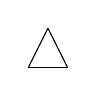
\begin{tikzpicture}[scale=0.5]
	\draw (0,0) -- (0.5,1);
	\draw (0,0) -- (1,0);
	\draw (0.5,1) -- (1,0);	
\end{tikzpicture} is big for $H = $
\begin{tikzpicture}[scale=0.5]
\draw (1,0) -- (0.5,1);
\end{tikzpicture}
using two colors. In the example, however it is possible to take edges of $G$ so that it remains big. $G =\;$
\begin{tikzpicture}[scale=0.5]
\draw (0.5,1) -- (1,0);
\draw (0,0) -- (1,0);
\end{tikzpicture}
and $G = $
\begin{tikzpicture}[scale=0.5]
\draw (1,0) -- (0.5,1);
\end{tikzpicture} are both big. The number of vertices of the smallest big graph is called Ramsey Graph Number. The example given is denoted by \ramGraph{H,H}.

More generally, however, each color can have its own target graph $H_{c_i}$ so the notation used is \ramGraph{H_1,\ldots,H_{|\colorset|}}.
However, in the special case that every target is a complete graph $K_{n_i}$, the amount of vertices in the smallest possible big graph is called Ramsey Number, instead of Ramsey Graph Number, and is denoted by $R(n_1, \ldots, n_{|\colorset|})$. 

The existence of big graphs for all target graphs and sets of colors is known since 1928 \todo{CITE On a problem of formal logic}, but the algebraic and computational challenges are yet to be solved. Ramsey Theory has many focuses of research, but one, is special, tends to the importance of knowing $G$ before the coloring process starts. That segment is called Online Ramsey Theory.

\subsection*{Online algorithms}

A well known online algorithm is the Canadian Traveler Problem. One tries to move from one city to another with bad whether conditions, making the connecting roads unpredictable. Using graph theoretical vocabulary, it is the problem of finding the shortest path between two vertices in a weighted directed graph, with one additional detail. At each step starting from the initial position, only the weight of the outgoing edges of the current vertex are known. That causes differences in the problem complexity when compared to the offline version solvable by Dijkstra's algorithm. 

\subsection*{Online Ramsey Theory}

The online version of the graph coloring problem studied in Ramsey theory is presented in different ways. Consider the following versions:

\begin{version}{1}
:Take a graph $G = K_n$ and a target $H$. Left and Right alternate coloring the edges of $K_n$ blue and red, respectively. The first player to create a monochromatic copy of $H$ in $G$ wins. If neither player is able to create it and there are no more uncolored edges, the game is a tie.
\end{version}

\begin{version}{2}
:Take a graph $G$ with no edges and a target $H$. Left selects two disconnected vertices of $G$ and adds an edge between them. Following, Right decides with what color to paint that edge. If a monochromatic copy of $H$ is ever created, then Left wins. It is common to allow $G$ to have an infinite amount of vertices, and consider that Right only wins if it provides a strategy to avoid $H$ indefinitely. In this version, Left and Right are typically called Builder and Painter, respectively.
\end{version}

Both versions are online as decisions are taken, either selecting, building or coloring edges, without knowledge of their consequences. For the remainder of this text version number two will be used and that is a matter of better matching the reference texts. Online algorithmic versions of the problem are typically referred to as Ramsey Games, Online Ramsey Theory and Online Ramsey Games.

The impact of the lack of information in the online version of the problem is significant. Pavel Dvo\v{r}\'ak shows in his master thesis \todo{cite his thesis} a very nice example, that was within reach since 2004, when the base theorem was proved in the paper ``On-line Ramsey Theory" \todo{cite text -> is in proposal too}. Consider the target is $P_3 = $
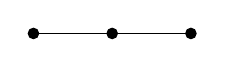
\begin{tikzpicture}
\begin{scope} [every node/.style={scale=0.4, circle, draw, fill=black}]
	\node (p1) at (0,0){};
	\node (p2) at (1,0){};
	\node (p3) at (2,0){};
\end{scope}
\draw (p1) -- (p2);
\draw (p2) -- (p3);
\end{tikzpicture}
. Now take $G =$
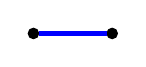
\begin{tikzpicture}
	\begin{scope} [every node/.style={scale=0.4, circle, draw, fill=black}]
		\node (p1) at (0,0){};
		\node (p2) at (1,0){};
	\end{scope}
	\draw[blue, ultra thick] (p1) -- (p2);
\end{tikzpicture}
. It is clear that in the next iteration $G^{LR} = G_1 =$
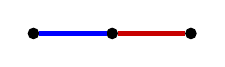
\begin{tikzpicture}
\begin{scope} [every node/.style={scale=0.4, circle, draw, fill=black}]
	\node (p1) at (0,0){};
	\node (p2) at (1,0){};
	\node (p3) at (2,0){};
\end{scope}
\draw[blue, ultra thick] (p1) -- (p2);
\draw[red, ultra thick] (p2) -- (p3);
\end{tikzpicture}
. Since $G_1$ is reachable, then so are  \hbox{$G_2 =$
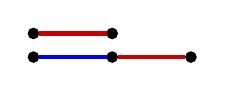
\begin{tikzpicture}
	\begin{scope} [every node/.style={scale=0.4, circle, draw, fill=black}]
		\node (p1) at (0,0){};
		\node (p2) at (1,0){};
		\node (p3) at (2,0){};
		\node (p4) at (0,0.3){};
		\node (p5) at (1,0.3){};
	\end{scope}
	\draw[blue, ultra thick] (p1) -- (p2);
	\draw[red, ultra thick] (p2) -- (p3);
	\draw[red, ultra thick] (p4) -- (p5);
\end{tikzpicture}}
and $G_3 =$
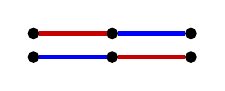
\begin{tikzpicture}
	\begin{scope} [every node/.style={scale=0.4, circle, draw, fill=black}]
		\node (p1) at (0,0){};
		\node (p2) at (1,0){};
		\node (p3) at (2,0){};
		\node (p4) at (0,0.3){};
		\node (p5) at (1,0.3){};
		\node (p6) at (2,0.3){};
	\end{scope}
	\draw[blue, ultra thick] (p1) -- (p2);
	\draw[red, ultra thick] (p2) -- (p3);
	\draw[red, ultra thick] (p4) -- (p5);
	\draw[blue, ultra thick] (p5) -- (p6);
\end{tikzpicture}
. Finally, by connecting either the left or the right ends of the two components, \hbox{$G^L_3 =$
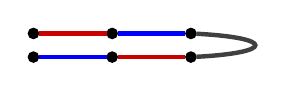
\begin{tikzpicture}
	\begin{scope} [every node/.style={scale=0.4, circle, draw, fill=black}]
		\node (p1) at (0,0){};
		\node (p2) at (1,0){};
		\node (p3) at (2,0){};
		\node (p4) at (0,0.3){};
		\node (p5) at (1,0.3){};
		\node (p6) at (2,0.3){};
	\end{scope}
	\draw[blue, ultra thick] (p1) -- (p2);
	\draw[red, ultra thick] (p2) -- (p3);
	\draw[red, ultra thick] (p4) -- (p5);
	\draw[blue, ultra thick] (p5) -- (p6);
	\draw[ultra thick, darkgray] (p3) to[out=3,in=-3, distance=1cm] (p6);
\end{tikzpicture}}.
In $G_4$, the gray edge would be colored either blue nor red. Therefore, Left would win. However,consider the following recoloring of \hbox{$G_4$, $G^*_4 = $

\begin{tikzpicture}
	\begin{scope} [every node/.style={scale=0.4, circle, draw, fill=black}]
		\node (p1) at (0,0){};
		\node (p2) at (1,0){};
		\node (p3) at (2,0){};
		\node (p4) at (0,0.3){};
		\node (p5) at (1,0.3){};
		\node (p6) at (2,0.3){};
	\end{scope}
	\draw[blue, ultra thick] (p1) -- (p2);
	\draw[red, ultra thick] (p2) -- (p3);
	\draw[blue, ultra thick] (p4) -- (p5);
	\draw[red, ultra thick] (p5) -- (p6);
	\draw[blue, ultra thick] (p3) to[out=3,in=-3, distance=1cm] (p6);
\end{tikzpicture}}. 

What prevented Right from getting that valid recoloring instead of the defeat in $G_4$ was not knowing Left's next moves. If Right knew Left would connect the right corners of the two stripes from the beginning, then Right would have colored the top edge, in $G^L_2$, blue and not red.

\subsection*{Restricting G}

The main challenge and focus of study in Ramsey Theory is finding Ramsey numbers. A challenge in Online Ramsey Games is, similarly, finding the smallest number of turns necessary for Left to win. However, there are other questions like the minimum number of edges a graph must have in order to be big as well or finding required substructures. An additional source of problems, in both areas, is deciding the outcomes of restricting the domain to particular classes of graphs. 

As per the first part of the introduction, it is true that there exists a big graph $G$ for every target $H$ and color set \colorset in Ramsey games. Consider, on the other hand, the class $\mathcal{G}$ to be the class of bipartite graphs. If Left can only build graphs in $\mathcal{G}$, then a triangle would, of course, be unreachable, therefore it does not have big graphs. However, knowing whether every bipartite graph is unavoidable or, equivalently, knowing if $\mathcal{G}$ is self-unavoidable, makes up a harder problem.

\subsection*{Planar Graphs}

Graphs that can be drawn without crossing edges form a class that is most typical of graph theory. Without the crossing edges, graph images becomes much easier to parse and that makes up for great visualization handicaps. They form a specially nice class instance for Ramsey games because, although these games are mostly concerned with combinatorial and computational questions, visualizing them allows both human interaction and algorithm inspection.

Over the past twenty years great progress has been made in terms of finding self-unavoidable sub-classes and discovering more of the overall impacts this restriction causes to Ramsey games. The next sections of the text focus on bringing initial results and recent developments for planar graphs. Following, a new game will be proposed.














    
    \chapter{Status}
    This section collects results of the Online Ramsey Game where both $G$ and $H$ are restricted to planar graphs. The first part of the section brings results from \textit{On-line Ramsey Theory}\todo{cite}, the paper that originated this study. The second part brings advancements made on \textit{Online Ramsey Theory for Planar Graphs}\todo{cite}. The section ends with extracts from \textit{Online Ramsey theory for a triangle on $F$‐free graphs}\todo{cite} that raises some questions on key subgraphs used by the Left in its strategy.

1st part:

The class of forests is self-unavoidable.

C3 is avoidable on the class of outerplanar graphs.

C3 in unavoidable on the class of planar 2-degenerate graphs.

Every cycle is unavoidable on planar graphs.

$K4\setminus \{e\}$ is unavoidable on planar graphs.

Conjecture 

2nd part:

Conjecture is wrong. $\Rightarrow$, but no $\Leftarrow$. Long proof and too many details to cover shortly. Find a way to simplify or only show key points and refer text...

Conjecture

3rd:

Say what F-Free is

Show result (when it is unavoidable and when it is not)

Raise question "For a given target $H$ and colorset $\mathcal{C}$, is there a finite collection of sets of graphs $\mathcal{F} = \{\mathcal{S}_1, \ldots, \mathcal{S}_n\}$ such that the builder needs all of $\mathcal{S}_i$ and no other graphs, other then their subdivisions, to make $H$ unavoidable"? 

If there is, what is the minimum number of forbidden subgraphs to make $H$ avoidable?
    
    \chapter{Exploring blindness}
    Up to this point the rules of Ramsey games were Left selecting two disconnected vertices and adding an edge between them and Right coloring it with a color from a predefined set of colors. There is a great difference between results of self-unavoidability and values for Ramsey numbers and Online Ramsey numbers. This difference comes from the lack of knowledge the Right player has, so making Right stronger might close that gap.

In the version presented so far, in each round Left adds an edge and Right colors that edge. Consider, instead, that Left adds two connected edges and Right colors both in their turns. This version is better for Right as it has more information to work with before coloring. However it is not clear if this handicap is enough to close the gap, nor if it makes any significant difference.

Taking k to be the number of edges in the connected component added and colored each turn, denote each version of the Online Ramsey Game to be k-Online Ramsey.

\begin{claim} {1}
:The class $\mathcal{G}$ is unavoidable in $1$-Online Ramsey $\iff$ $\mathcal{G}$ is unavoidable in $k$-Online Ramsey for any positive integer $k$.
\end{claim}
\begin{claim} {2}
:Take $f_k(G, (H_1, \ldots, H_c))$ to be the function that maps a $k$-Online Ramsey game to its respective number. Then, 
$$f_k(G, (H_1, \ldots, H_c)) = g(k) \cdot f_1(G, (H_1, \ldots, H_c))$$
with \mbox{$g \in O(1)$}. Same as saying that the additional information makes no significant difference.
\end{claim}

Evidence:

Consider the theorem by Grytczuk, Haluszczak and Kierstead that the class of forests is self-unavoidable in the $1$-Online Ramsey with $2$ colors. The same property applies to any $k$-Online Ramsey, with the same proof.

Proposition:

The class of forests is self-unavoidable in k-Online Ramsey.

Proof:

It suffices to prove the assertion for trees. Let $T$ be any tree with $n$ vertices $v_i, \ldots, v_n$. We apply induction on the number of vertices. Let $u$ be a leaf of $T$ and let $T' = T - u$. By induction the Builder can force $n$ disjoint copies of $T_1, \ldots, T_n$ of $T'$ in the same color.
Now, in each of the following $n$ rounds, the Builder adds an edge $(u_i, u_j)$, for $u_i \in V(T_i)$ and $u_j \in V(T_j)$ the vertices adjacent to the corresponding vertex $u$ removed. Builder also adds edges $(u_i, v_1), \ldots, (u_i, v_k-1)$, with $v_i$ any vertex disconnected from all trees, in its turn. Regardless of the Painter decision, when the last edge $(u_i, u_j)$ is colored, a monochromatic $T$ is created.

Note that both claims are supported. Claim 2 is supported as the Builder build $k-1$ additional edges in each round, incrementing the total number of needed vertices by a constant factor of $k-1$.



    
    \appendix
    \chapter{Appendix A}
    

\end{document}
%----------------------------------------------------------------------------------------------------%
